\section{实验步骤}

本章节将描述实验步骤,包括概要设计和详细设计。

\subsection{概要设计}

\subsubsection{总体架构}

本章节将展示该系统的总体架构。

\begin{figure}[H]
    \centering
    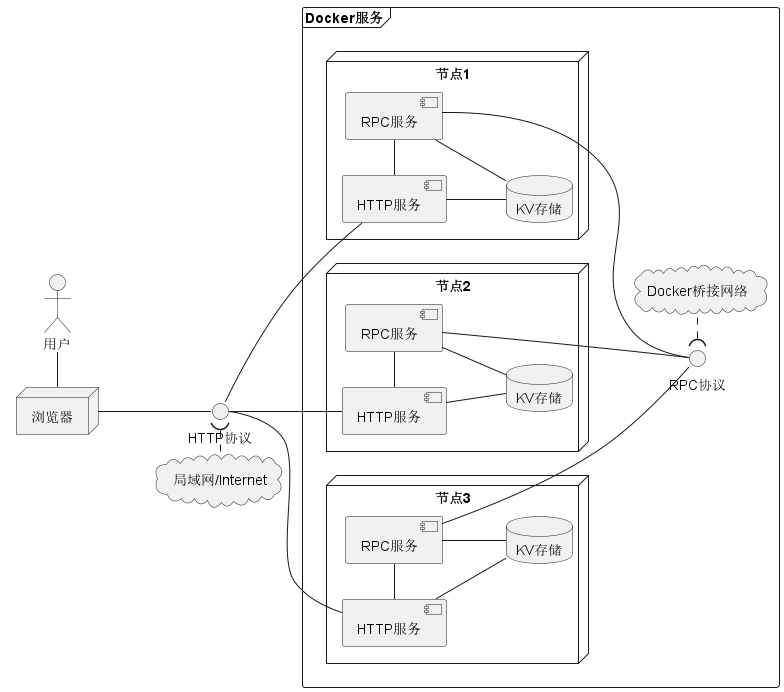
\includegraphics[width=\linewidth]{examples/总体架构.png}
    \caption{总体架构}
    \label{fig:arch}
\end{figure}

如图\ref{fig:arch}所示,该系统的总体架构是B/S架构,用户可通过浏览器,基于HTTP协议,通过局域网或Internet与服务端进行交互,服务端对用户来说完全透明。

服务端内部则是分布式架构,不同节点拥有独立业务逻辑,能够完成完整的数据存储和读取业务。节点通过HTTP服务接收用户请求,之后与本地的KV存储进行交互来完成数据的存取。

当节点数量不只有1个时,节点之间就可以通过RPC服务进行通信。当请求通过哈希函数分配给本机时,节点会自行处理逻辑,否则就会通过RPC发送给目标节点进行处理,并接收其返回值再返回到用户。节点之间通过Docker桥接网络进行通信。

\subsubsection{模块设计}

本章节将展示该系统的模块设计。

\begin{figure}[H]
    \centering
    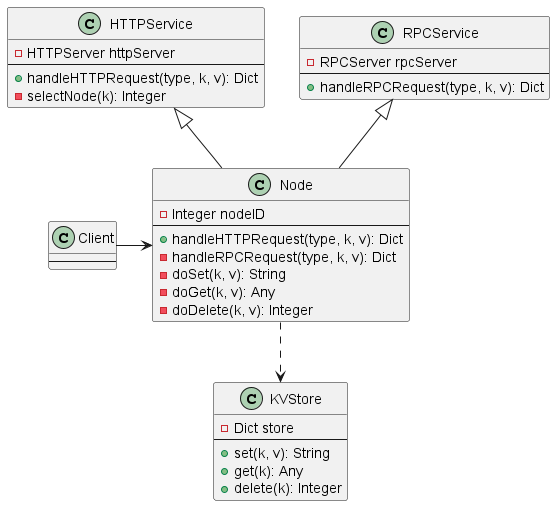
\includegraphics[width=0.8\linewidth]{examples/模块设计.png}
    \caption{模块设计}
    \label{fig:modules}
\end{figure}

如图\ref{fig:modules}所示,本系统可分为4个模块:
\begin{itemize}
    \item HTTP服务(HTTPService)。该模块负责接收的HTTP请求,并选择处理请求节点。
    \item RPC服务(RPCService)。该模块负责接收并处理RPC请求。
    \item KV存储(KVService)。该模块负责存储和读取键值对。
    \item 节点(Node)。通过Python多继承的特性,该模块负责整合所有模块并合理选择处理逻辑。如果请求节点属于本节点,该模块会调用本地的设置、获取、删除等处理函数;否则,将通过RPC调用目标节点的处理函数。
\end{itemize}